\documentclass[a4paper, 12pt]{article}
% For fonts
% \usepackage{palatino}
% \usepackage[T1]{fontenc}
% \usepackage{mathpazo}
% \usepackage{textcomp}
% \usepackage{fouriernc}
% \usepackage{mathastext}
\usepackage[scaled = 0.9]{scholax}


\usepackage{setspace}
\usepackage{amsmath}%
\usepackage{amssymb}%
\usepackage{mathtools}
\usepackage{dsfont}
\DeclareMathOperator*{\argmax}{arg\,max}
\DeclareMathOperator*{\argmin}{arg\,min}



\usepackage[table]{xcolor}%




\setlength{\marginparwidth}{6cm}
\usepackage{todonotes}
\usepackage[in]{fullpage}%
%\usepackage{enumitem}

\usepackage{amsthm}

\usepackage{titlesec}%
\titlelabel{\thetitle.\hspace{0.5em}}%
\usepackage{xcolor}%
\usepackage{mleftright}
\usepackage{xspace}%
\usepackage{graphicx}
\usepackage{float}
\usepackage{hyperref}%
\usepackage{etoolbox}
\usepackage{lipsum}
\usepackage{appendix}
\usepackage{tikz}
\usepackage{mathrsfs}
\usepackage{listings}
\usepackage{enumitem}
% \usepackage[normalem]{ulem}
\usepackage[nameinlink,noabbrev]{cleveref}
% Math font, must be loaded after amsmath
\usepackage[scaled = 0.95,varbb]{newtxmath}
\usepackage{booktabs}
\usepackage{threeparttable}
\usepackage[natbibapa]{apacite}
\usepackage{subcaption}

\usepackage{hyperref}%
\hypersetup{%
unicode,
breaklinks,%
colorlinks=true,%
urlcolor=blue,%
linkcolor=[rgb]{0.5,0.0,0.0},%
citecolor=[rgb]{0,0.2,0.445},%
filecolor=[rgb]{0,0,0.4},
anchorcolor=[rgb]={0.0,0.1,0.2}%
}

\newenvironment{thmenum}{%
\begin{enumerate}[label=\small(\alph*\small),topsep=4pt,itemsep=4pt,partopsep=0pt, parsep=0pt]
}{%
\end{enumerate}
}

\newtheoremstyle{break}
  {\topsep}{\topsep}%
  {\itshape}{}%
  {\bfseries}{}%
  {\newline}{}%
\theoremstyle{break}
\newtheorem{theorem}{Theorem}[section]

\theoremstyle{break}
\newtheorem{lemma}[theorem]{Lemma}

\theoremstyle{break}
\newtheorem{corollary}[theorem]{Corollary}

\theoremstyle{break}
\newtheorem{proposition}[theorem]{Proposition}

\theoremstyle{break}
\newtheorem{definition}[theorem]{Definition}

\theoremstyle{break}
\newtheorem{assumption}[theorem]{Assumption}


\theoremstyle{break}
\newtheorem*{remark}{Remark}

\theoremstyle{break}
\newtheorem*{example}{Example}

\newtheorem{innercustomthm}{Exercise}
\newenvironment{exercise}[1]{\renewcommand\theinnercustomthm{#1}\innercustomthm}{\endinnercustomthm}

\newenvironment{solution}{\begin{proof}[Solution]}{\end{proof}}

\renewcommand\qedsymbol{\rule{2mm}{2mm}}
\usepackage{setspace}
\setstretch{1.2}
\usepackage{appendix}

\title{\large{Career Pathways: Advanced Study or Immediate Work}}
\author{Yin-Yun Li}
\date{December, 2024}




\begin{document}
\maketitle

\section{Introduction}

According to the Ministry of Interior in Taiwan, the proportion of the population with tertiary education has been increasing. In 2022, $42\%$ of young adults aged between 25 and 64 completed the highest level of education. 
Some attribute this trend to higher education reforms in Taiwan since $1990$s, which involved the extensive establishment of universities and made higher education more accessible to the younger generation. 
Others suggest that low tuition fees and school subsidies also play a role in shaping individuals' choices. 

In Taiwan, compulsory education spans ages 6 to 15. Most students then choose to enroll in senior high school for an additional three years. 
After completing the 12-year national education program, they can decide whether to pursue advanced study or enter the labor market directly.

We usually think that going to colleges helps us develop occupation-specific skills and earn higher wages in the labor market. 
However, identifying the causality is empirically challenging.
What factors affect a younger person's career choice? 
How is the cost of schooling measured?
To what extent does policy reform matter?

To answer these questions, we construct a simple dynamic discrete choice model to analyze a single agent's decision based on human capital, education cost and heterogeneous shock. 

\section{Related Literature}

Our model connects human capital and the return to education within a dynamic discrete choice framework. 
Human capital has been widely discussed in the literature, with education and experience being two of the most important forms of investment. 
\cite{becker1964human} observed that education level tends to be positively correlated to earnings, 
while \cite{mincer1974schooling} demonstrates years of experience rather than age, along with schooling, explains the wage differential.

To estimate the causal effect of returns to education, the reduced-form approach is the most common method. 
However, estimates from ordinary least squares (OLS) are often argued to be upward biased.
To address the endogeneity issue, \cite{angrist1991does} employed the quarter of birth as an instrument to support the evidence that longer compulsory schooling
results in higher wages, despite the insignificant difference between 2LSL and OLS estimators.
Later, \cite{angrist1992estimating} used the draft lottery to isolate the variation in school enrollment and found that
an additional year of schooling increases weekly earnings by 6.6 percent.
The similar positive relation is also documented in \cite{card1993using}.
All these studies suggest little evidence of ability bias in conventional OLS estimates.
\cite{card1999causal, card2001estimating} show that marginal returns to education are shaped more by supply-side factors---particularly the marginal cost of schooling---than by low ability.

\cite{willis1979education} adopted a structural model approach to support the hypothesis that expected earnings influence the decision to attend college.
Positive selection at two levels of schooling echoes comparative advantage rather than ability bias.
In the dynamic framework, \cite{keane1997career} developed a dynamic human captial investment model to analyze schooling, work, and occupational decisions of the younger generation in the U.S. 
The model provides an excellent fit to observed data, including lifetime decisons and wage profiles.
Concurrently, \cite{belzil1997estimating} proposed an optimal stopping model that incorporates learning costs, parental support, school ability, and labor market ability. 
The specification also captures non-wage benefits as a key determinants in career decisions.

In the context of Taiwan, \cite{Hsu2021HigherEd} used Heckman's two-stage selection model combined with a difference-in-differences strategy to validate the college expansion lowers the wages of university graduates.
In contrast, \cite{Li2009ReturnsEducationTaiwan} leveraged the Panel Study of Family Dynamics (PSFD) with 2SLS, HT, and panel GMM to construct consistent estimators, finding an insignificant negative effect on returns as college enrollment rates increased.
\cite{ChuangLai2011CohortEducation} employed quantile regression to estimate heterogeneous returns to education across birth cohorts,
but the underlying mechanisms remain unexplored due to data limitations.

To our knowledge, few studies have examined career paths and wage accumulations of young adults in Taiwan.
We hope this basic human capital model can serve as a starting point for understanding the dynamic patterns and offering insights into education and labor market policy.

\section{The Model}

Let us start with a simple single-agent discrete choice model. Assume people only care about monetary factors. 
Each individual $i$ faces a finite horizon problem from age $t=18$ to $T=30$. The flow payoff function is:
\begin{equation}
U(X_{it},\varepsilon_{it}, a_{it}) =
\begin{cases}
    \log \left(1+\beta_1 s_{it} + \beta_2 x_{it}\right) + \varepsilon_{it}(1) & \text{if } a_{it} = 1 \\
    \qquad \quad\;\, -C\cdot x_{it} + \varepsilon_{it}(0) & \text{if } a_{it} = 0,
\end{cases}
\end{equation}

where \(U(.)\) is the flow utility, 
$s$ represents years of tertiary education, and $x$ denotes occupational experience.
The term $\varepsilon_{it}$ is an idiosyncratic shock across time and individuals, which is observed only by the agent.
The opportunity cost of education, $C$, depends on the current level of occupational experience.
That is, the cost of forgoing earnings to pursue further education rises as work experience accumulates.


The law of motions for $s$ and $x$ evolves as follows: 
\begin{equation}
\begin{split}
x_{t+1} &= x_t + \mathds{1}{\{a_t=1\}}, \quad \forall t; \\
s_{t+1} &= s_t + \mathds{1}{\{a_t=0\}},\quad s \leq \bar{s},\;t\leq 30.
\end{split}
\label{law_of_motion}
\end{equation}

Before the age of 30, if the agent chooses to work, occupational experience increases by 1 while years of schooling remain unchanged. Conversely, if the agent chooses to study, years of schooling increase by 1 while occupational experiences remain the same.
Note that \(\bar{s}\) denotes the maximum years of higher education, which we set to 12 for simplicity.


Our wage process follows the Mincer equation:
\begin{align}
w_{it}= \beta_0+\beta_1 s_{it}+\beta_2 x_{it} + \beta_3 x^2_{it} +  \xi_{it},
\label{mincer}
\end{align}


The intercept term, $\beta_0$, represents the fixed skill endowment and the baseline wage offer with only a high school degree and no work experience.
The coefficent of quadratic term, $\beta_3$, reflects the diminishing marginal returns of experience on earnings and is expected to be negative.
The $\beta_1, \beta_2$ are the two main parameters of interest. To avoid identification issue, we normalize $\beta_0 = 1$ and $\beta_3=0$.

The error term, $\xi_{i} \overset{\text{i.i.d.}}{\sim} N(0, \sigma^2_{\xi})$, is the heterogeneity of productivity across individual. 
Since employers in the labor market cannot observe the error term, they pay each employee (i.e., agent) the average earnings conditional on personal state:
\begin{equation}
E[w_{it}|X_{it}] = X_{it}^{\prime}\beta,
\end{equation}

where $X_{it}=[1, s_{it}, x_{it}],\,\beta=[1, \beta_1, \beta_2]'$.
Agents' choice set consists of two alternatives: pursuing a job ($a_{it} = 1$) and keeping studying ($a_{it} = 0$). 
When an individual decides to work, he can always find a job and receive a wage offer \(X_{it}^{\prime}\beta\); 
once an agent decides to pursue further education, they incur an opportunity cost of $C\cdot x_{it}$, 
which may include forgone earnings or college tuition.
We also assume there are no friction between the labor market and schooling.

Let $\delta \in (0,1)$ be the discount factor. At each period $t$, agents aims to maximize the lifetime expected utility by choosing $a_{it}\in\{0,1\}$:
\begin{equation}
\max_{a_t \in \{0,1\}}\mathbb{E} \bigg(  \sum_{\tau=0}^{T-t} \delta^{\tau} \{u(X_{t+\tau}, a_{t+\tau}) + \varepsilon_{t+\tau}(a_{t+\tau})\} \mid  X_{t},\varepsilon_t, a_{t} \bigg).
\label{bellman_eq}
\end{equation}

Note that we ignore the subscript $i$ since every agent follows the same decision rule. Rewrite the maximization problem as Bellman equation:
\begin{equation}
\small
V(X_{t}, \varepsilon_t) = \max_{a_{t} \in \{0,1\}} \bigg[ u( X_{t}, a_t) +  \varepsilon_{t}(a_{t}) + \delta \iint V(X_{t+1}, \varepsilon_{t+1})dG(\varepsilon_{it}) dF(X_{t+1} \mid X_{t},a_{t})\bigg].
\end{equation}


\subsection{Identification}
The solution to this basic model involves in computing the optimal lifetime decision paths $\{a_t^*\}^T_{t=18}$ for each agent.
Our goal is to recover the deep parameters $\{\beta_1, \beta_2, C, \delta, \sigma_{\xi} \}.$
In the basic model, we only focus on the first three parameters and calibrate the discount factor at $\delta = 0.95$. 
Recall that agents in our model receive only average earnings. 
Although this assumption is somewhat unrealistic simplification, 
it allows us to sidestep the difficult task of estimating ability heterogeneity.

Following \cite{rust1987optimal}, we assume the unobservable component $\varepsilon_{it}$ follows Type I Extreme Value (T1EV) distribution, 
and we can define an integrated value function in the state of $X_{t}$ before the realization of random shock:
\begin{equation}
\Bar{V}(X_t) = \int_\varepsilon V(X_t,\varepsilon_t)g(\varepsilon_t) d\varepsilon_t = \mathbb{E}_\varepsilon \left[ V(X_t, \varepsilon_t) \right] .
\end{equation}

By Assumption \eqref{as2}, the integrated value function can be derived as:
\begin{equation}
\label{eq_barv}
\begin{split}
\mathbb{E}_\varepsilon \left[ V(X_t, \varepsilon_t) \right] &= \mathbb{E}_\varepsilon \left[ \max_{a_t} \left\{ \varepsilon(a_t) + u(X_t, a_t) + \delta \mathbb{E}\left(V(X_{t+1}, \varepsilon_{t+1}) \right)\right\} \right]\\
&= \ln \left\{ \sum_{a_t} \exp \left( u(X_t, a_t) +\mathbb{E}_{X_{t+1}} [\Bar{V}(X_{t+1})|X_{t}, a_t] \right) \right\} + \gamma,
\end{split}
\end{equation}

where $\gamma$ is Euler-Mascheroni constant.

Note that in equation \eqref{eq_barv}, we can define the choice-specific value function which does not depend on $\varepsilon_t$:
\begin{equation}
\begin{split}
v(X_{t}, a_t) &\equiv u(X_t, a_t) + \delta\int \Bar{V}(X_{t+1}) df(X_{t+1} \mid X_{t}, a_t)dX_{t+1}\\
&= u(X_{t}, a_{t}) + \delta \mathbb{E}_{X_{t+1}} [\Bar{V}(X_{t+1})|X_{t}, a_t].
\end{split}
\end{equation}


Last, we can derive the conditional choice probability (CCP) of choosing action $a_t$ given state $X_t$:
\begin{equation}
\begin{split}
\Pr(a_t=j\mid s_t, x_t) &= \Pr(v_j+\xi(j)>v_k+\xi(k), k\neq j\mid s_t, x_t)\\
&= \frac{\exp(v_j)}{\exp(v_1)+\exp(v_0)}, \quad j,k\in\{0,1\}, 
\label{ccp}
\end{split}
\end{equation}

where $s\in[0,12]$ and $x\in[0,12]$.

\subsection{Data Generation Process}
Individuals’ decision process begins at age 18, after graduating from senior high school. 
In each period, they draw two independent random shocks from the T1EV distribution and compute the lifetime expected reward associated with each option. 
After comparing the two alternatives, agents choose the action that yields the higher utility and update the state variables according to \eqref{law_of_motion}. 

For simplicity, we assume that after the age of 30, all agents exclusively choose to work. 
At this stage in life, schooling no longer increases job earnings, and the option to study is no longer available. 
Consequently, the decision to work becomes an absorbing state, as agents remain in this state for the remainder of their lives, with occupational experiences increasing by one each period.

Table \eqref{summ_stat} documents an overview of the descriptive statistics from the simulated data.
At the aggregated level, most individuals choose to work,
while only a few opt to pursue higher education, with the maximum years of schooling reaching 9.

Figure \eqref{fig:decision_by_age} shows the probability of choosing higher education versus entering the labor market by age. 
Monotonic patterns are observed for both choices: individuals are more likely to attend college at younger ages,
and they gradually enter the workforce after completing the studies.
\begin{table}[hpbt]
\centering
\begin{tabular}{lcccc}
\toprule
& mean    & min & median & max \\ 
\cmidrule(lr){2-5}
years of higher education & 2.2474 & 0 & 2  & 9  \\
\addlinespace
work experiences   & 3.7526 & 0  & 3   & 12  \\ 
\addlinespace
\% choosing to work    & 79.823\%    & -      & -   & -   \\ 
\bottomrule
\end{tabular}
\caption{Summary Statistics (N = 30000)}
\label{summ_stat}
\end{table}

\begin{figure}[] 
    \centering
    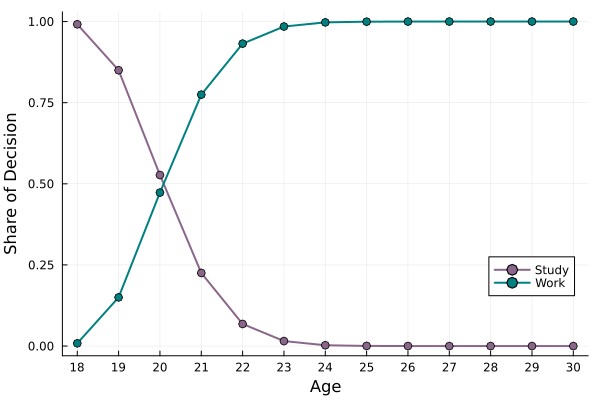
\includegraphics[width=0.85\textwidth]{decision_by_age.png}
    \caption{Age Profile of Study and Work Decisions}
    \label{fig:decision_by_age}
\end{figure}




\section{Estimation}
\subsection{NFXP}
Given the simulated data, we use nested fixed point (NFXP) algorithm to back up the parameters of the model. 
The algorithm consists of two loops. 
We begin with an initial set of arbitrary parameters, $\hat\theta_0=\{\hat\beta_1, \hat\beta_2, \hat{C}\}$, 
and solve $\bar V(X_t; \hat\theta_0)$ in \eqref{eq_barv} via value function iteration, which helps us construct the CCP in \eqref{ccp}. 
In the outer loop, we use maximum likelihood estimation to update the parameters to $\hat\theta_1$. The process proceeds iteratively until convergence.
The likelihood function is:
\begin{equation}
    \mathcal{L}(\theta\mid X_{it}, a_{it}) 
    = \prod_{n=1}^N\prod_{t=18}^{30}\prod_{j=1}^2\Pr(a_{it}=j\mid X_{it})^{\mathbf{1}\{a_{it}=j\}}.
    \label{likelihood_func}
    \end{equation}



\subsection{Preliminary Results}
Table \eqref{est_paras} summarizes the predetermined parameters and the estimation results.
\begin{table}[hpbt]
\centering
\begin{tabular}{llcc}
\toprule
& & predetermined value & estimates \\
\cmidrule{2-4}
Schooling Effect & $\beta_1$ & 3.6 & 3.674 \\
\addlinespace
Work Experiences Effect & $\beta_2$ & 1.79  & 1.821 \\ 
\addlinespace
Cost of Schooling & $C$ & 2.58 & 2.561 \\
\bottomrule
\end{tabular}
\caption{Estimates of Model Parameters}
\label{est_paras}
\end{table}


\section{Policy Experiment}
In this section, we use the estimated model to conduct a policy experiment.
Suppose the government implements a subsidy program of the fixed amount $S=1.5$ to encourage individuals to pursue higher education.
The flow utility function is modified as follows:
\begin{equation}
U(X_{it},\varepsilon_{it}, a_{it}) =
\begin{cases}
    \log \left(X_{it}\beta\right) + \varepsilon_{it}(1) & \text{if } a_{it} = 1 \\
    S-C\cdot x_{it} + \varepsilon_{it}(0) & \text{if } a_{it} = 0,
\end{cases}
\end{equation}

and individuals solve the Bellman equation in \eqref{bellman_eq} with this new flow utility function.

Figure \eqref{fig:subsidy_effect_on_decision} shows that the subsidy policy provides a strong incentive 
for individuals to pursue higher education, leading to a higher probability of completing master's or PhD degrees.
The monotonic patterns remain: once individuals enter
the labor market, they are unikely to return to school.

Figure \eqref{fig:wage_profile_comparison} compares the lifetime utility, as characterized by wage profiles, under the estimated model and the counterfactual scenario.
With the subsidy, more individuals attain tertiary education and accumulate additional years of schooling.
This leads to an upward shift in the wage profile since schooling effect in our model is larger than the experience effect ($\beta_1>\beta_2$).
However, the policy's effectiveness should be discussed with caution, as this basic model does not account for the government's budget and the potential social cost.

\begin{figure}[h] 
    \centering
    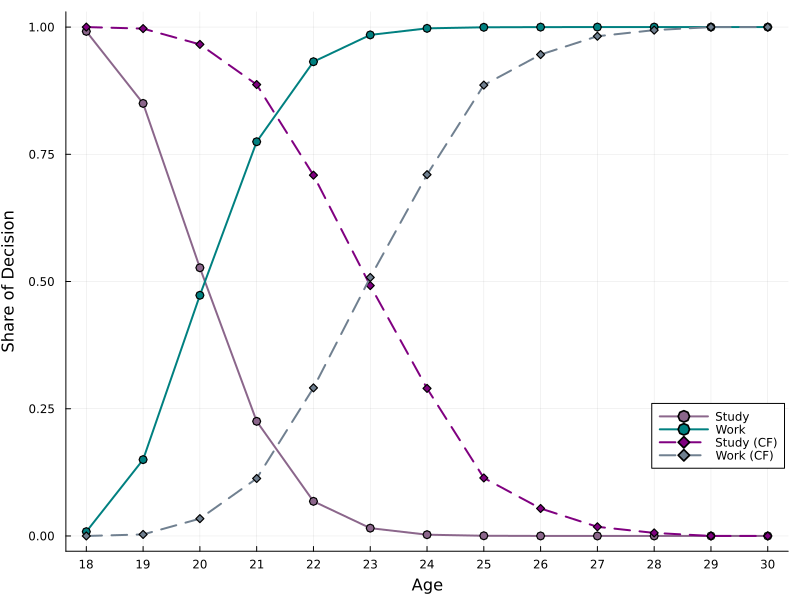
\includegraphics[width=0.85\textwidth]{decision_by_age_comparison.png}
    \caption{Age Profile of Study and Work Decisions: Baseline v.s. Counterfactual}
    \label{fig:subsidy_effect_on_decision}
\end{figure}

\begin{figure}[h] 
    \centering
    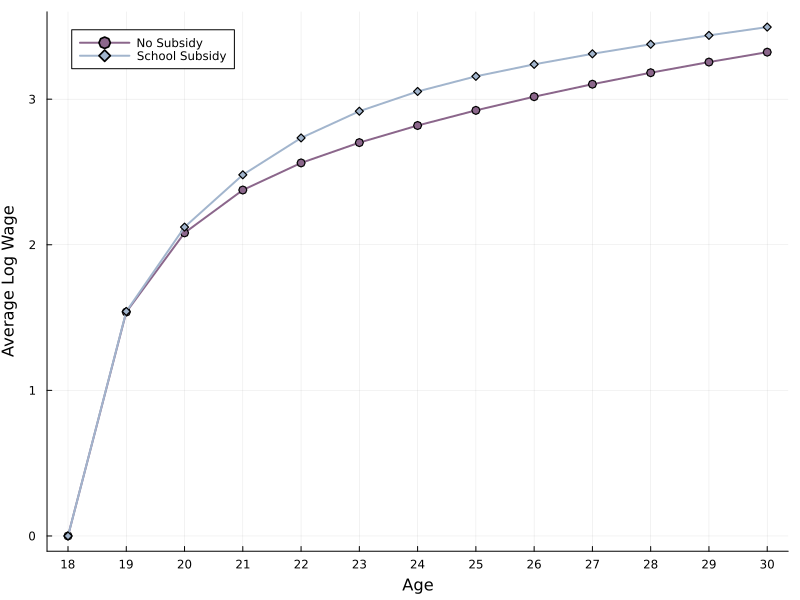
\includegraphics[width=0.85\textwidth]{lifetime_utility.png}
    \caption{Wage Profile: Baseline v.s. Counterfactual}
    \label{fig:wage_profile_comparison}
\end{figure}


\clearpage
\appendix
\section{Rust Assumptions}
We follow the standard assumptions in \cite{rust1987optimal} to solve the dynamic discrete choice model.

\begin{assumption}[Additive Separability]
The one-period utility function is additively separable:
\begin{equation}
   U( X_{it},\varepsilon_{it}, a_{it}; \beta) = u(X_{it}, a_{it}; \beta) + \varepsilon_{it}(a_{it}).
\end{equation}
\label{as1}
\end{assumption}

\begin{assumption}[IID T1EV shocks]
The unobserved components are i.i.d. across alternatives, agents and time with T1EV CDF \( G(.) \); The unobserved shocks are contemporarily independent of \( X_{it} \):
\begin{equation}
\begin{split}
 \varepsilon_{it}(a_{it}) &\overset{\textit{iid}}{\sim}  G_{\varepsilon}(\varepsilon_{it})\\
X_{it} &\perp \varepsilon_{it}. 
\end{split}
\end{equation}
\label{as2}
\end{assumption}


\begin{assumption}[Conditional Independence of Future States; CI-X]
The future state \( \{ X_{it+1}, \varepsilon_{it+1} \}\) depends only on the current state and action:
\begin{equation}
\begin{split}
   P(X_{it+1}, \varepsilon_{it+1} \mid X_{it}, a_{it}, \varepsilon_{it}) &= P(X_{it+1}, \varepsilon_{it+1} \mid X_{it}, a_{it}) \\&=F_X(X_{it+1} \mid X_{it}, a_{it})G(\varepsilon_{it+1}) 
\end{split}
\end{equation}
\label{as3}
\end{assumption}

Note that in the second equality we use the Assumption \eqref{as2}.

\begin{assumption}[Discrete Support of \( X_{it} \); DIS]
The state variables \( X_{it} \) (years of schooling $\boldsymbol{s}$ \& occupational experience $\boldsymbol{x}$) have a discrete and finite support:
\begin{equation}
    X_{it} \in \{X^{(1)}, X^{(2)}, \dots, X^{(|X|)}\}, \quad |X| < \infty.  
\end{equation}
\label{as4}

That is, 
\begin{equation}
s_{it},\, x_{it}\in\{0,1,2,...,12\}.
\end{equation}
\end{assumption}

\clearpage
\bibliographystyle{apacite}
\bibliography{ref}
\end{document}
